% Options for packages loaded elsewhere
\PassOptionsToPackage{unicode}{hyperref}
\PassOptionsToPackage{hyphens}{url}
%
\documentclass[
]{book}
\usepackage{lmodern}
\usepackage{amssymb,amsmath}
\usepackage{ifxetex,ifluatex}
\ifnum 0\ifxetex 1\fi\ifluatex 1\fi=0 % if pdftex
  \usepackage[T1]{fontenc}
  \usepackage[utf8]{inputenc}
  \usepackage{textcomp} % provide euro and other symbols
\else % if luatex or xetex
  \usepackage{unicode-math}
  \defaultfontfeatures{Scale=MatchLowercase}
  \defaultfontfeatures[\rmfamily]{Ligatures=TeX,Scale=1}
\fi
% Use upquote if available, for straight quotes in verbatim environments
\IfFileExists{upquote.sty}{\usepackage{upquote}}{}
\IfFileExists{microtype.sty}{% use microtype if available
  \usepackage[]{microtype}
  \UseMicrotypeSet[protrusion]{basicmath} % disable protrusion for tt fonts
}{}
\makeatletter
\@ifundefined{KOMAClassName}{% if non-KOMA class
  \IfFileExists{parskip.sty}{%
    \usepackage{parskip}
  }{% else
    \setlength{\parindent}{0pt}
    \setlength{\parskip}{6pt plus 2pt minus 1pt}}
}{% if KOMA class
  \KOMAoptions{parskip=half}}
\makeatother
\usepackage{xcolor}
\IfFileExists{xurl.sty}{\usepackage{xurl}}{} % add URL line breaks if available
\IfFileExists{bookmark.sty}{\usepackage{bookmark}}{\usepackage{hyperref}}
\hypersetup{
  pdftitle={Using LANDFIRE Products to explore historical and current ecosystems},
  pdfauthor={The Nature Conservancy's LANDFIRE team},
  hidelinks,
  pdfcreator={LaTeX via pandoc}}
\urlstyle{same} % disable monospaced font for URLs
\usepackage{longtable,booktabs}
% Correct order of tables after \paragraph or \subparagraph
\usepackage{etoolbox}
\makeatletter
\patchcmd\longtable{\par}{\if@noskipsec\mbox{}\fi\par}{}{}
\makeatother
% Allow footnotes in longtable head/foot
\IfFileExists{footnotehyper.sty}{\usepackage{footnotehyper}}{\usepackage{footnote}}
\makesavenoteenv{longtable}
\usepackage{graphicx,grffile}
\makeatletter
\def\maxwidth{\ifdim\Gin@nat@width>\linewidth\linewidth\else\Gin@nat@width\fi}
\def\maxheight{\ifdim\Gin@nat@height>\textheight\textheight\else\Gin@nat@height\fi}
\makeatother
% Scale images if necessary, so that they will not overflow the page
% margins by default, and it is still possible to overwrite the defaults
% using explicit options in \includegraphics[width, height, ...]{}
\setkeys{Gin}{width=\maxwidth,height=\maxheight,keepaspectratio}
% Set default figure placement to htbp
\makeatletter
\def\fps@figure{htbp}
\makeatother
\setlength{\emergencystretch}{3em} % prevent overfull lines
\providecommand{\tightlist}{%
  \setlength{\itemsep}{0pt}\setlength{\parskip}{0pt}}
\setcounter{secnumdepth}{5}
\usepackage{booktabs}
\usepackage[]{natbib}
\bibliographystyle{plainnat}

\title{Using LANDFIRE Products to explore historical and current ecosystems}
\author{The Nature Conservancy's LANDFIRE team}
\date{2021-02-16}

\begin{document}
\maketitle

{
\setcounter{tocdepth}{1}
\tableofcontents
}
\hypertarget{landfire-for-landscape-ecosystem-assessment}{%
\chapter{LANDFIRE for landscape ecosystem assessment}\label{landfire-for-landscape-ecosystem-assessment}}

There are some basic steps in assessing the ecological situation of your landscape, including:

\begin{itemize}
\tightlist
\item
  mapping historical and current ecosystems, and the difference between the two; and further looking at representation of ecosystems inside and outside of your landscape of interest.
\item
  assessing succession classes (aka seral states) of these ecosystems, past and present
\item
  understanding natural disturbance regimes
\end{itemize}

These steps, while foundational and conceptually simple can be difficult due to a lack of data, especially when doing then at a landscape scale which often means looking across multiple land ownerships.

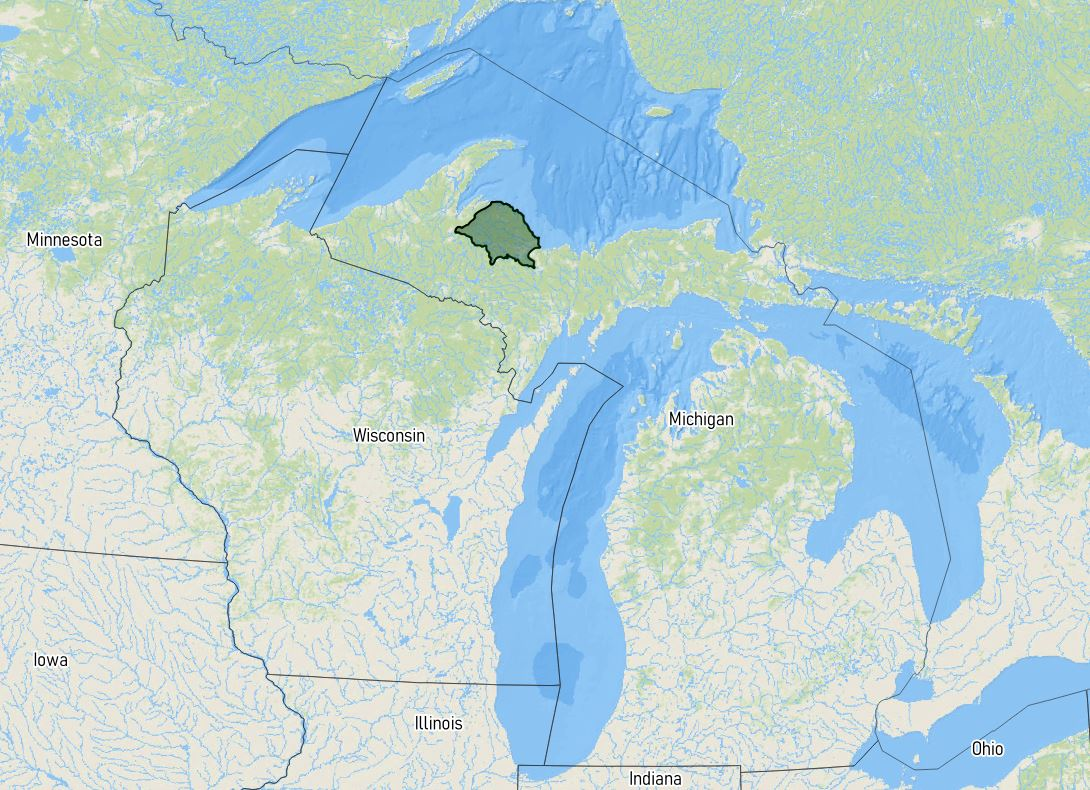
\includegraphics[width=15.67in]{mh_locator}

In the United States, including the insular areas \href{www.landfire.gov}{LANDFIRE} provides the datasets and ecological model results to get at these challenges and more. Here we walk you through some of the technical steps needed to start your analysis. We will do our work in a model landscape, the Michigamme Highlands in the Upper Peninsula of Michigan (highlighted in green in map).

This is a technical guide-we will provide links for you to learn about the datasets and other inputs.

\hypertarget{softAndData}{%
\chapter{Software and Datasets}\label{softAndData}}

\hypertarget{to-get-started-you-will-need-the-landfire-products.-the-hyperlined-text-will-lead-you-to-descriptions}{%
\section{To get started you will need the LANDFIRE products. The hyperlined text will lead you to descriptions:}\label{to-get-started-you-will-need-the-landfire-products.-the-hyperlined-text-will-lead-you-to-descriptions}}

\begin{itemize}
\tightlist
\item
  Spatial datasets, clipped to your area(s) of interest

  \begin{itemize}
  \tightlist
  \item
    \href{https://www.landfire.gov/bps.php}{Biophysical Settings (BpS)}. This dataset will be used to get at ``community habitat'', or where ecosystems could occur based on abiotic factors (e.g., soils, climate).
  \item
    \href{https://www.landfire.gov/sclass.php}{Succession classes} characterizes structural classes on the landscape at the time the dataset represents (e.g., 2016 for LF Version 200).
  \item
    \href{https://www.landfire.gov/evt.php}{Existing Vegetation Type} maps NatureServe's Ecological Systems (see descriptions \href{https://www.landfire.gov/documents/LANDFIRE_Ecological_Systems_Descriptions_CONUS.pdf}{here}).
  \end{itemize}
\item
  Non-spatial products

  \begin{itemize}
  \tightlist
  \item
    \href{http://landfirereview.org/search.php}{Biophysical Settings Descriptions} which has information on natural disturbance regimes and succession class descriptions (also available \href{https://tnc.box.com/s/d3ocvy969s1792m5885filjhktujp86e}{here}).\\
  \item
    \href{https://tnc.box.com/s/d3ocvy969s1792m5885filjhktujp86e}{Reference Condition Table} supplements the BpS descriptions with the ``reference'' percentages for each succession class, for each Biophysical Settings.
  \end{itemize}
\end{itemize}

\hypertarget{guidance-on-obtaining-landfire-products}{%
\section{Guidance on obtaining LANDFIRE products}\label{guidance-on-obtaining-landfire-products}}

There are multiple ways to get LANDFIRE depending on whether you are looking to obtain BpS models and descriptions or the spatial data:

\begin{itemize}
\item
  For BpS models and descriptions go to: \url{http://landfirereview.org/search.php}. Start by clicking on the ``View map of LANDFIRE Map Zones''. This will help you narrow down your search. Alternatively, you can wait to download BpS descriptions until you do some GIS work and get specific names of BpSs of interest.
\item
  For the spatial datasets you can explore options \href{https://www.landfire.gov/getdata.php}{here} which include:

\begin{verbatim}
  * Downloading [Full Extent Mosaics](https://www.landfire.gov/version_comparison.php).  When you do use this option you get large files that cover the entire lower 48, AK or HI (depending on your selection).  We use this method when we have several landscapes and/or a large area and no computer storage issues.
  * Using the [LANDFIRE Data Distribution Site](https://www.landfire.gov/viewer/).  With this method you essentially select the datasets you need then draw a rectangle (or you can select state or counties) around your area of interest to start the downloader.  We recommend this if your area of interest is not too large and/or you have a low number of landscapes and/or have storage limits.
\end{verbatim}
\end{itemize}

\hypertarget{gisPrep}{%
\chapter{GIS prep}\label{gisPrep}}

\hypertarget{combine-data}{%
\section{Combine data}\label{combine-data}}

Once spatial data is properly projected and clipped to area of interest, perform a ``combine'' in ArcMap (Toolbox \textgreater{} Spatial Analyst \textgreater{} Local \textgreater{} Combine) of the BpS, SCL and EVT datasets. Alternatively, you can combine a raster of the area of interest with those 3 datasets which are stored as larger extents (like shown below).

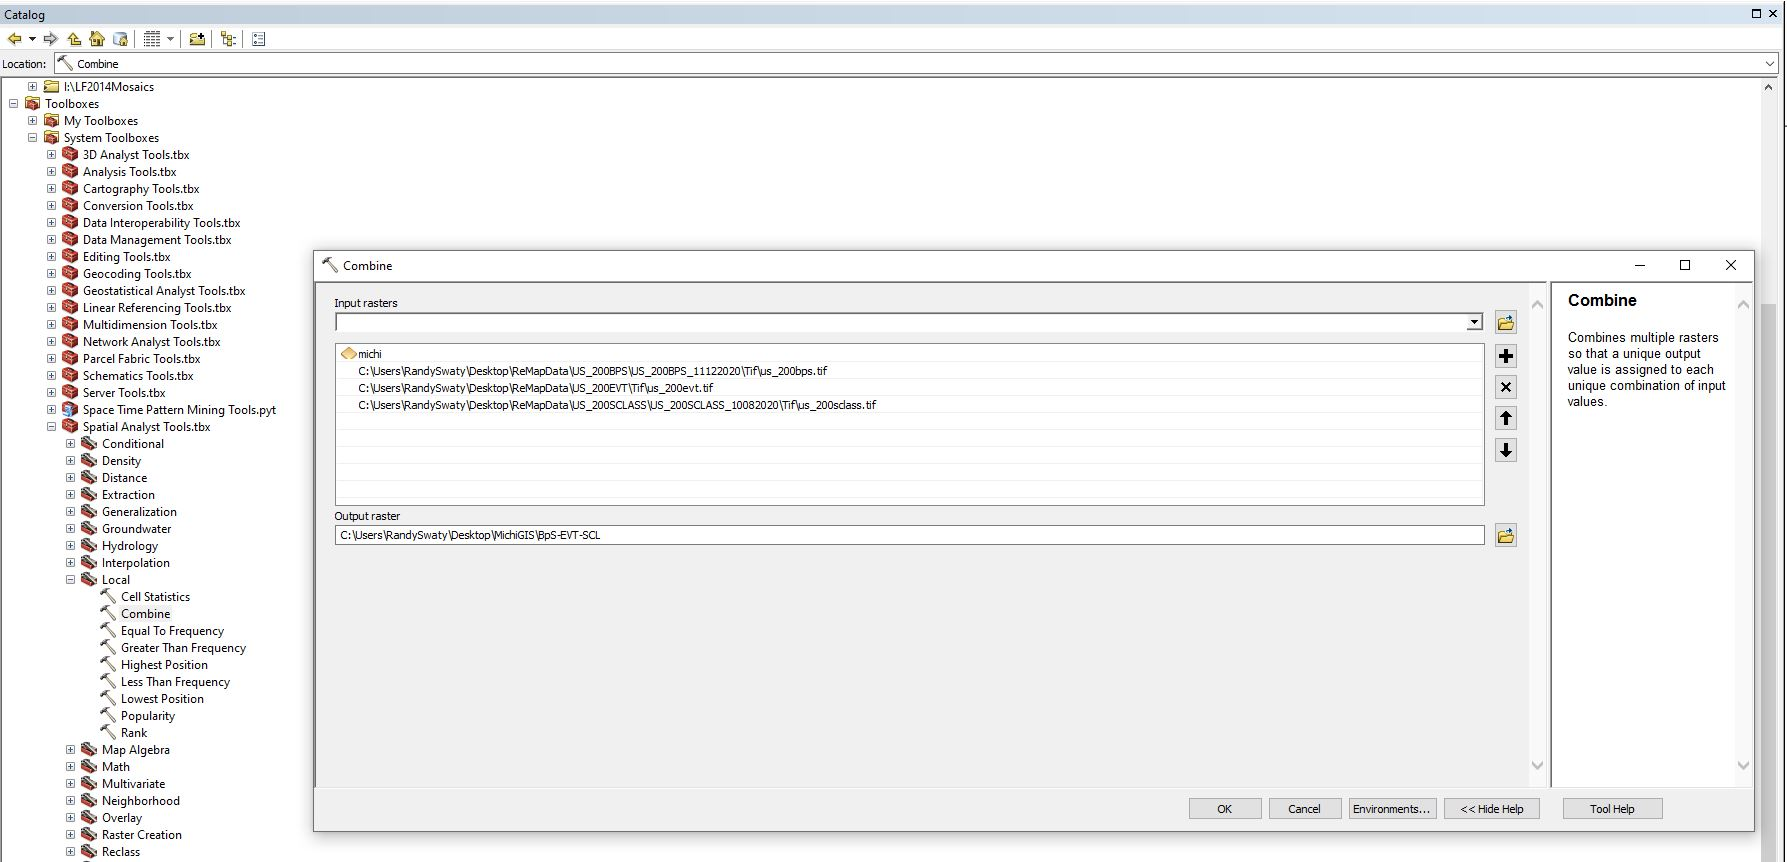
\includegraphics[width=1\linewidth]{combine}

\hypertarget{join-in-attributes}{%
\section{Join in attributes}\label{join-in-attributes}}

There are multiple ways-we recommend using the Join Field tool (Toolbox \textgreater{} data management tools \textgreater{} joins \textgreater{} add join). One reason to do this is to be able to select which fields to join in. A potential resulting table looks like this for a landscape in Michigan (with minimal cleaning/formatting):

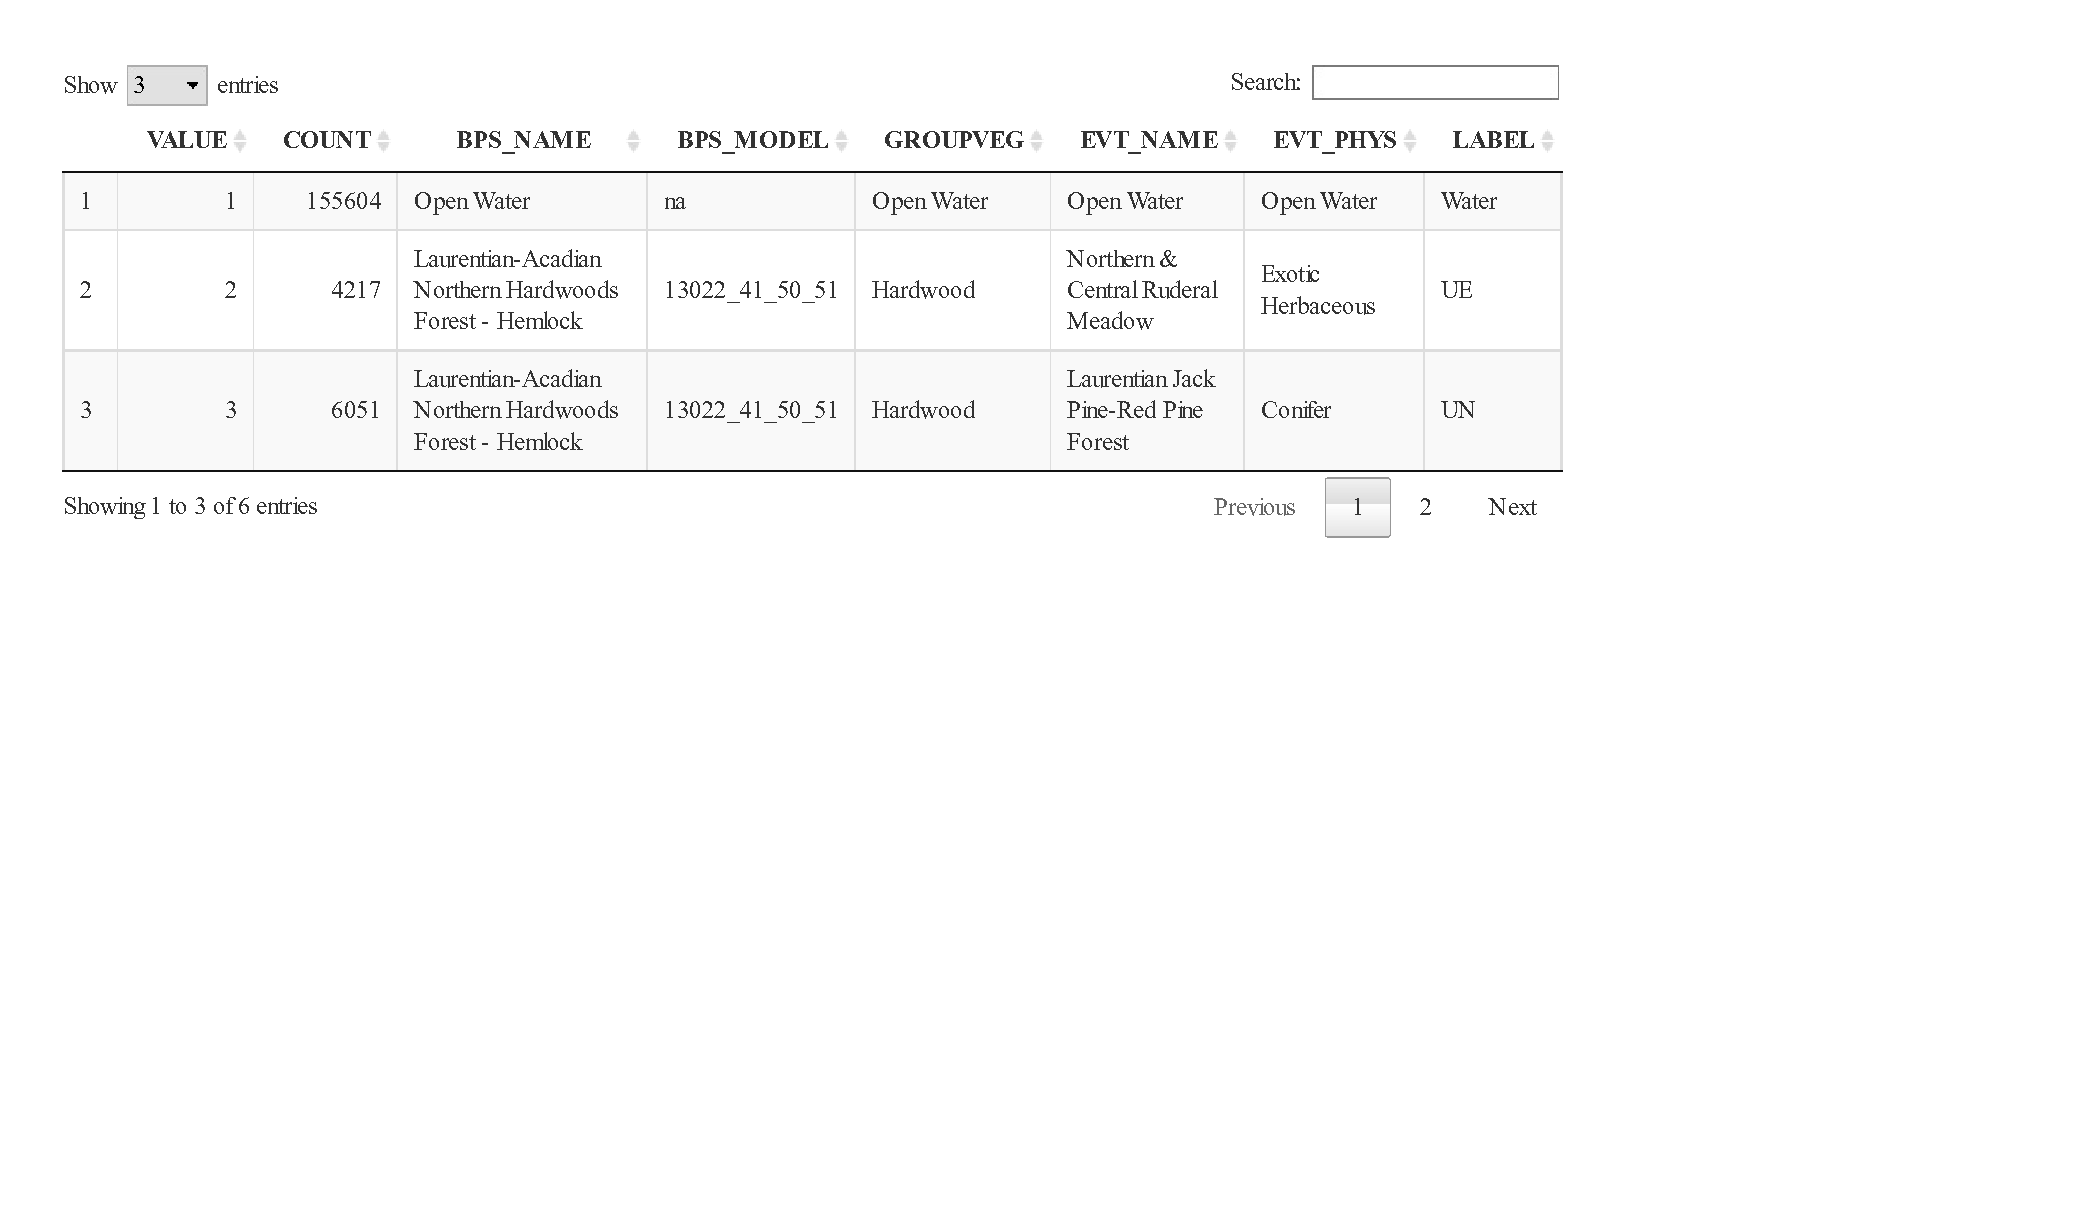
\includegraphics{FSCBook_files/figure-latex/combineDT-1.pdf}

As is this table does not mean too much-we will need to do some cleaning, formatting and calculating.

\hypertarget{clean-data-table}{%
\section{Clean data table}\label{clean-data-table}}

You will first need to save the combined ``.csv'' file file as an ``.xlsx'' file so that you can have multiple worksheets. We recommend keeping the original output as a ``raw'' spreadsheet in Excel, pasting that data into a new sheet and working with that new sheet moving forward.
* It is OK to remove the ``US\_200BPS'', ``US\_200EVT'', and ``US\_200SCLASS'' columns
* Rename some columns: ``GROUPVEG'' to ``BPSGROUPVEG''; ``EVT\_PHYS'' to ``EVTGROUPVEG''; ``LABEL'' to ``SUCCESSIONCLASS'', or similar as needed for clarity
* COUNT = number of 30m x 30m pixels for that combination of BpS-EVT-SCLS. Insert a column named ``ACRES'', then calculate acres by multiplying COUNT by ``0.222''. Copy-Paste Values for that new column. Below is an example of what our new data table looks like.

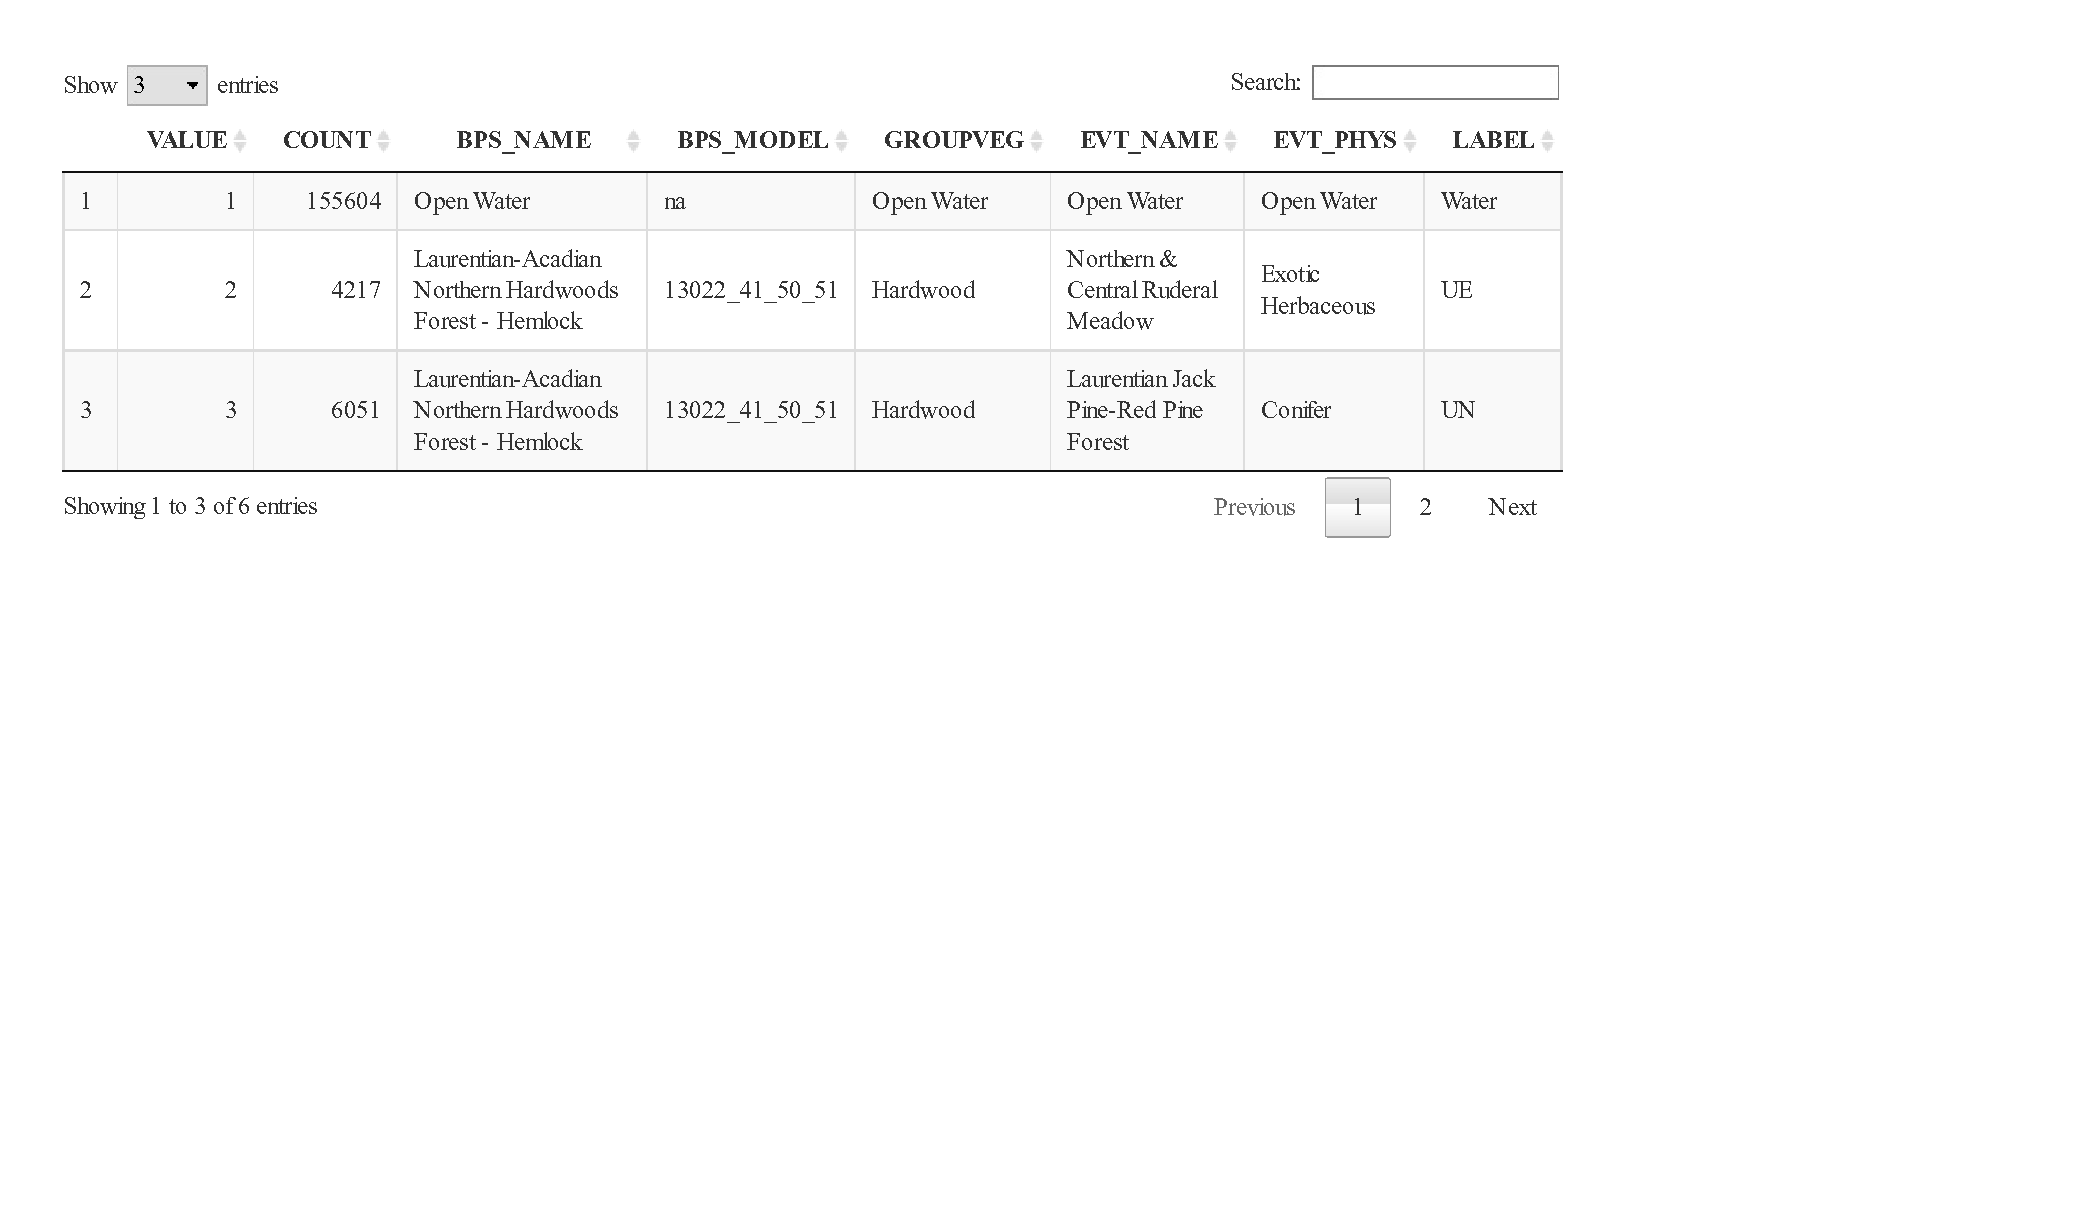
\includegraphics{FSCBook_files/figure-latex/combineCleanDT-1.pdf}

Now we are ready for some Pivot Table excitement!

\hypertarget{historicalEcosystems}{%
\chapter{Historical Ecosystems}\label{historicalEcosystems}}

In this chapter we will learn:

\begin{itemize}
\tightlist
\item
  Which ecosystems, and how much of each were on our landscape historically
\item
  How much of each ecosystem has been converted to other land uses (e.g., agriculture)
\item
  How much of each historical ecosystem is mapped as a different ecosystem as of the latest LANDFIRE dataset
\end{itemize}

\hypertarget{first-question-how-many-acres-what-percent-of-each-ecosystem-were-in-the-area-of-interest-historically}{%
\section{First Question: how many acres (what percent) of each ecosystem were in the area of interest historically?}\label{first-question-how-many-acres-what-percent-of-each-ecosystem-were-in-the-area-of-interest-historically}}

For the next few questions we will work in a Pivot Table. To get started copy the entire ``clean'' sheet, click ``Insert'' at in the Excel ribbon then click ``Pivot Table''. Once your pivot table is created you can start to explore.

\begin{enumerate}
\def\labelenumi{\arabic{enumi}.}
\tightlist
\item
  In the Pivot Table Fields pane, select BpS Name then acres.\\
\item
  Right click in the top ``Sum of ACRES'' field (not the table header), then sort in descending order.
\item
  In our example we have some BpSs that have low ACRES values. We also have categories that are not meaningful, such as ``Barren-Rock/Sand/Clay''. We can do a little formatting/cleaning before making a chart:

  \begin{itemize}
  \tightlist
  \item
    To remove BpSs from the table you will click the drop-down menu to the right of ``BPS\_NAME'' in the Pivot Table Fields pane. You can uncheck BpSs as appropriate.
  \item
    It is also possible to filter by right clicking on the top value in the list of BpSs, then selecting Filter \textgreater{} Top 10\ldots. Once in that menu you can refine the filtering.
  \end{itemize}
\item
  To get percentages, drag ``ACRES'' from the top Pivot Table Field pane to the ``Values'' pane. This will add a second ``ACRES'' column to the table. Click the drop down in the second instance of ``ACRES'' (reads ``SUM of ACRES2'' in our example), then Value Field Settings. In this menu select the ``Show Values As'' tab, click the ``Show Values As'' drop down then select ``\% of Grand Total\% to get percentages of each BpS (make sure that''BPS\_NAME" is selected as the ``Base field'').\\
\item
  To get a ``running total'' of percentages you will add a third instance of ``ACRES'' to the ``Values'' pane, then Value Field Settings. In this menu select the ``Show Values As'' tab, click the ``Show Values As'' drop down then select ``\% Running Total In'' to get running totals of percentages of each BpS (make sure that ``BPS\_NAME'' is selected as the ``Base field'').
\item
  Save and keep this pivot table as is for now. We will make a couple modifications in the next section to get at a different question.
\end{enumerate}

Formatted table of BpSs:

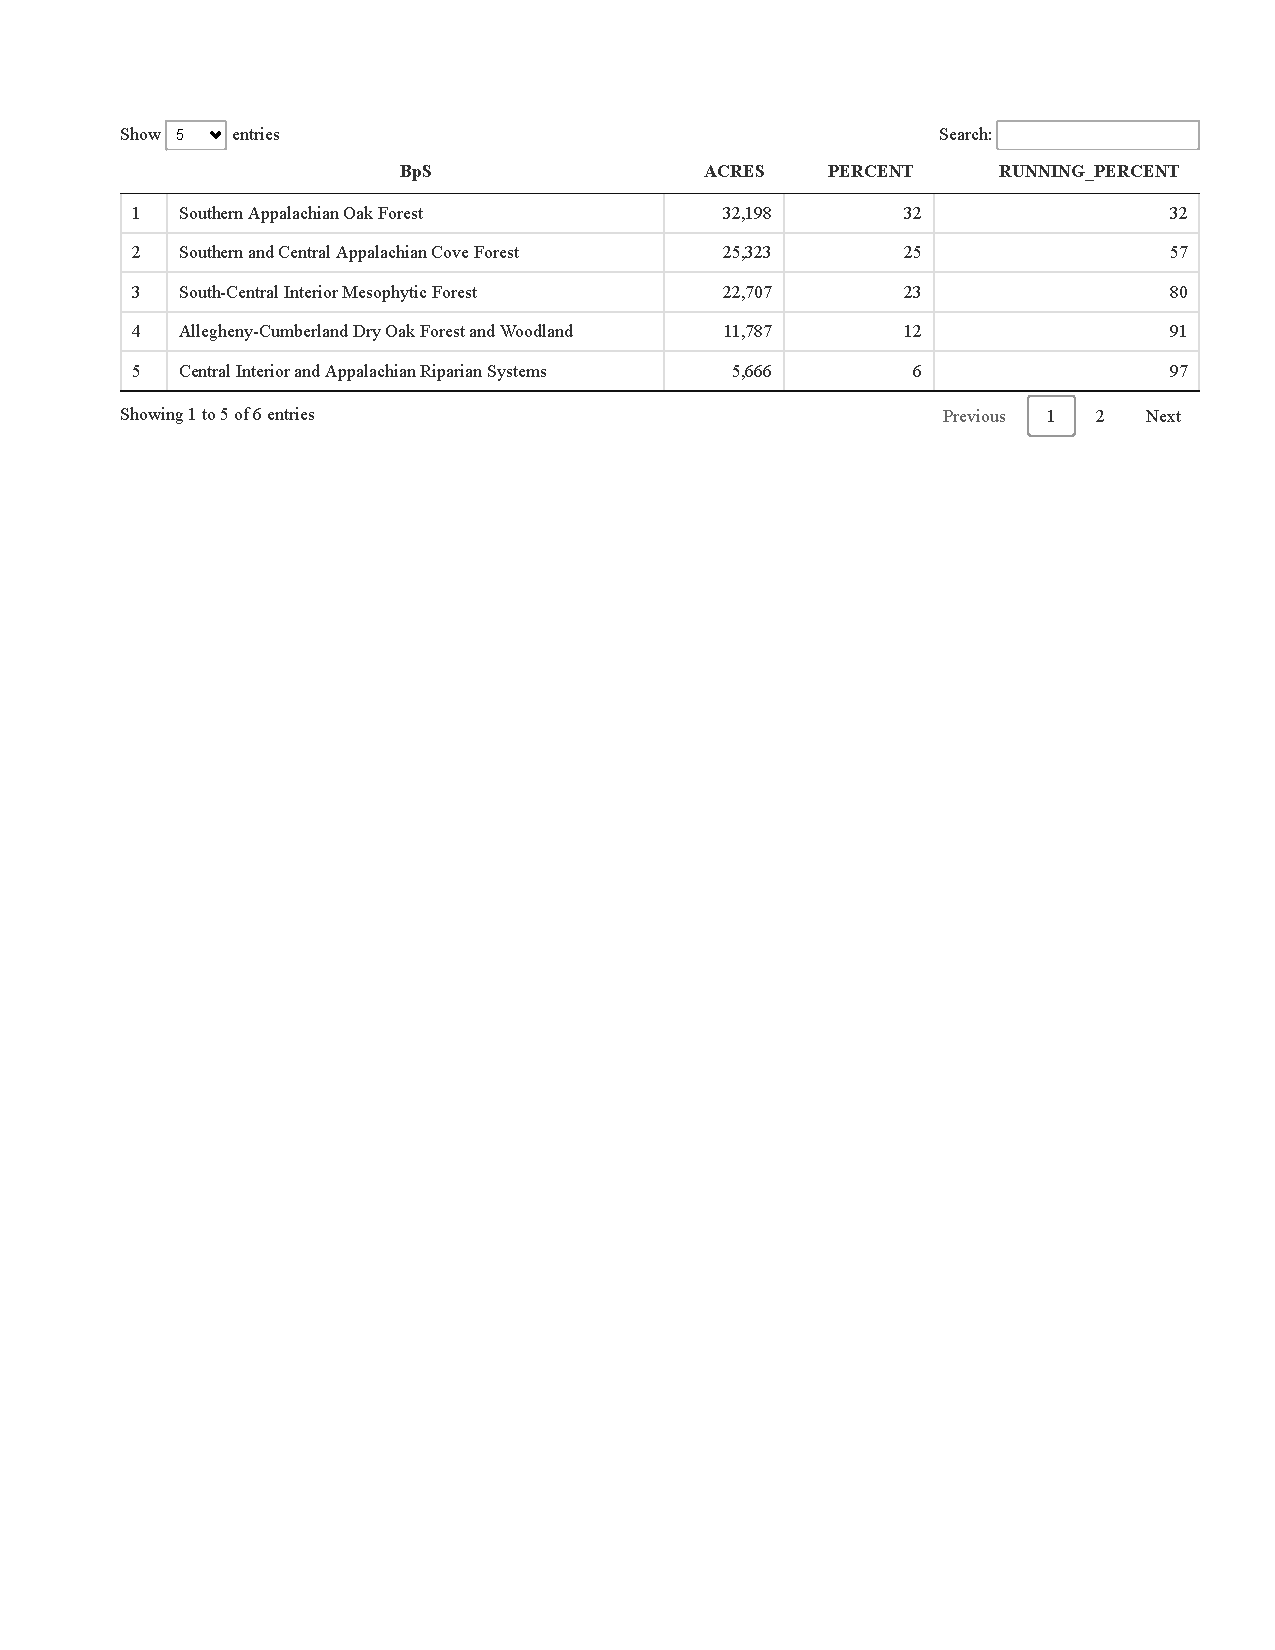
\includegraphics{FSCBook_files/figure-latex/bpsDT-1.pdf}

We see that the top 4 BpSs comprised \textasciitilde80\% of our example landscape historically. We can visually confirm this and other patterns with a quick chart made in R (though similar charts available in Excel):

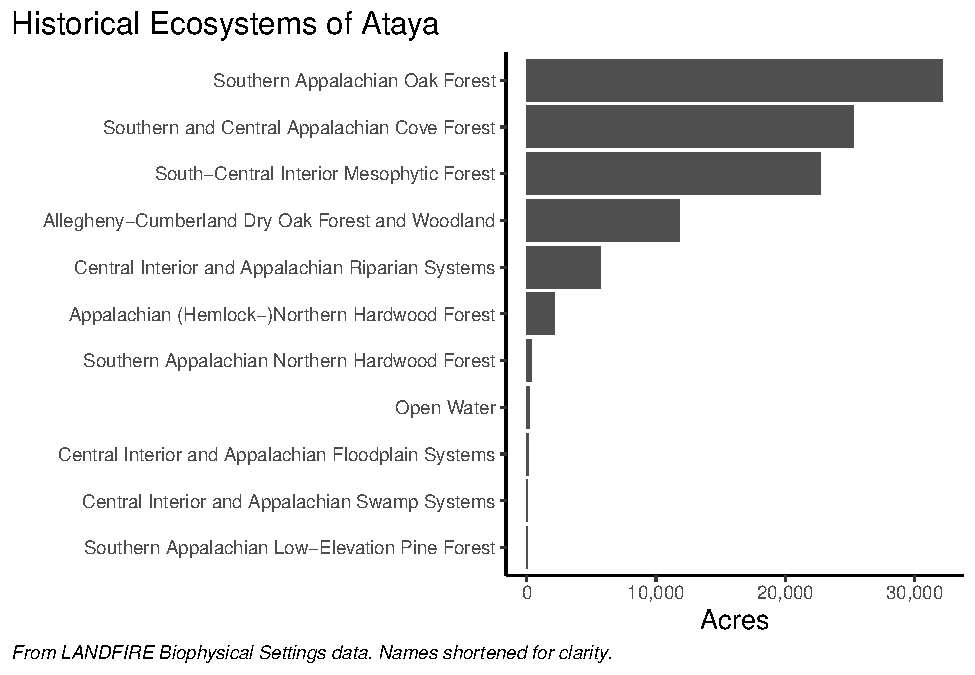
\includegraphics{FSCBook_files/figure-latex/bpsChart-1.pdf}

\hypertarget{second-question-how-much-of-the-historic-ecosystems-have-been-converted-to-a-different-land-use-e.g.-agriculture-or-have-succeeded-to-a-different-ecosystem}{%
\section{Second question: how much of the historic ecosystems have been converted to a different land use (e.g., agriculture), or have succeeded to a different ecosystem?}\label{second-question-how-much-of-the-historic-ecosystems-have-been-converted-to-a-different-land-use-e.g.-agriculture-or-have-succeeded-to-a-different-ecosystem}}

If you are new to Pivot Tables this next section will 1) demonstrate their power and 2) showcase ways they can mislead!

Working in the Pivot Table from before (or you can create a new one if you prefer):

\begin{enumerate}
\def\labelenumi{\arabic{enumi}.}
\tightlist
\item
  Check the box next to ``EVT\_NAME'' in the Pivot Table Fields pane. Make sure that everything is arranged as in the screenshot below (e.g., ``BPS\_NAME'' is on top of ``EVT\_NAME'' in the ``Rows'' pane). Note-I am about to sort in descending order.
\end{enumerate}

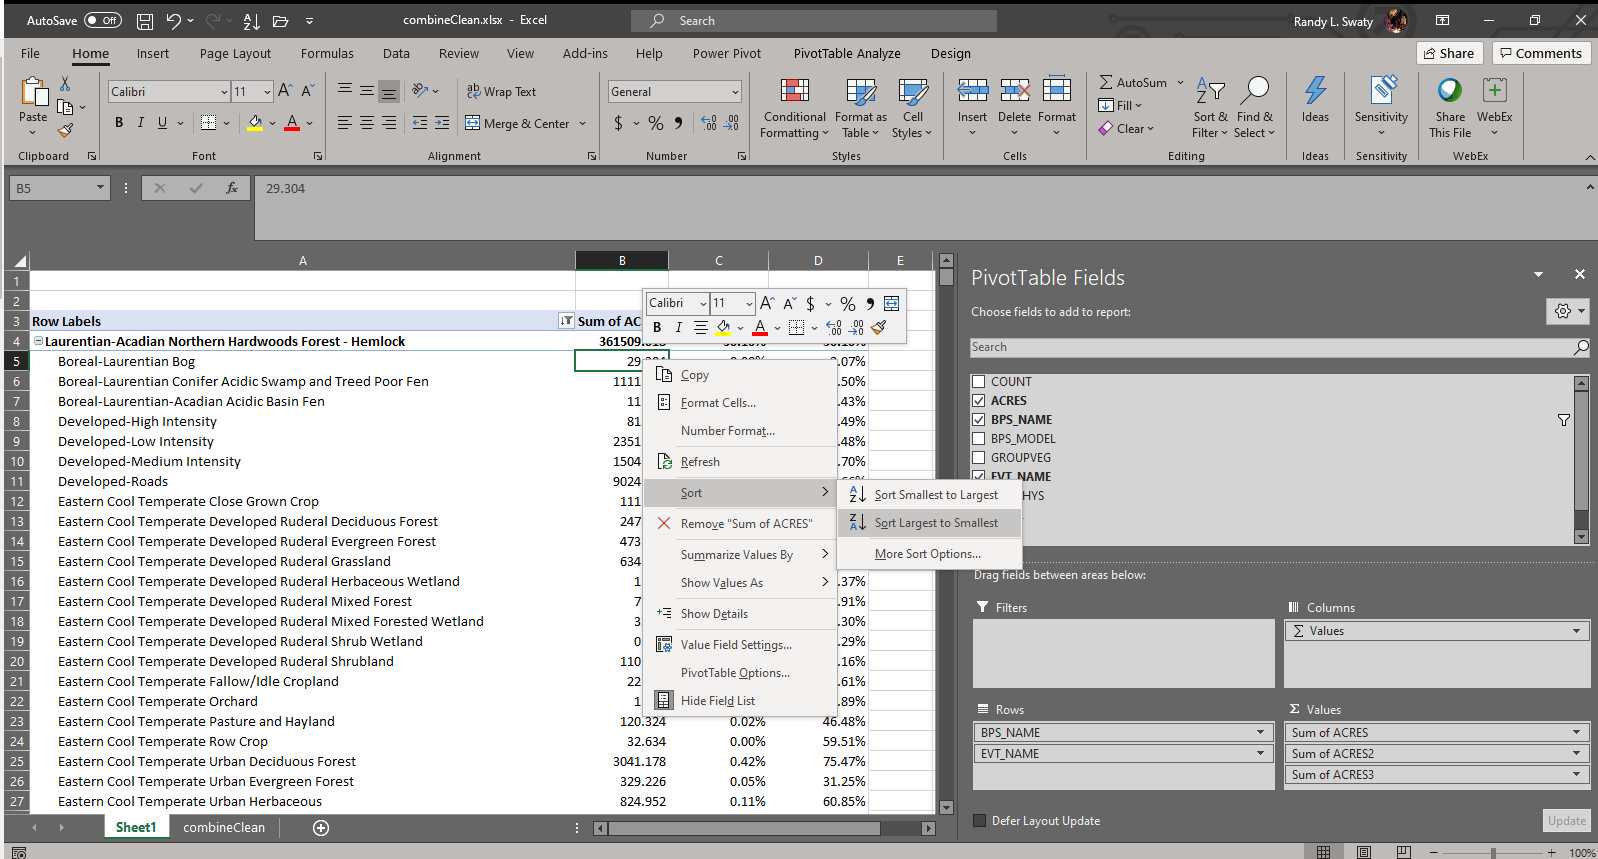
\includegraphics[width=1\linewidth]{pivotBpsEvt}

\begin{enumerate}
\def\labelenumi{\arabic{enumi}.}
\setcounter{enumi}{1}
\tightlist
\item
  Review the results. In the example above we can see that what LANDFIRE mapped as Laurentian-Acadian Forest-Hemlock in the BpS data set has been split into many Existing Vegetation Types. If ordered we get a little more information, but the numbers are misleading. We'd like to see how much of what was Ecosystem X is still Ecosystem X, and how much is now Ecosystem Y, and so on, but the numbers are looking across the whole landscape. They need to be recalculated so we get the percentage of EVT per BpS.
\item
  To reconfigure the Pivot Table:

  \begin{itemize}
  \tightlist
  \item
    Drag the ``Sum of ACRES2'' and ``Sum of ACRES3'' field from the ``Values'' pane up to the Pivot Table Fields to remove it.
  \item
    Click the ``Sum of ACRES'' item in the ``Values'' pane to access the Value field settings.
  \item
    Click on the ``Show Values As'' tab, then select ``\% of Parent Row Total'' in the ``Show Values As'' drop down.
  \end{itemize}
\end{enumerate}

Here's a screenshot of making that selection:

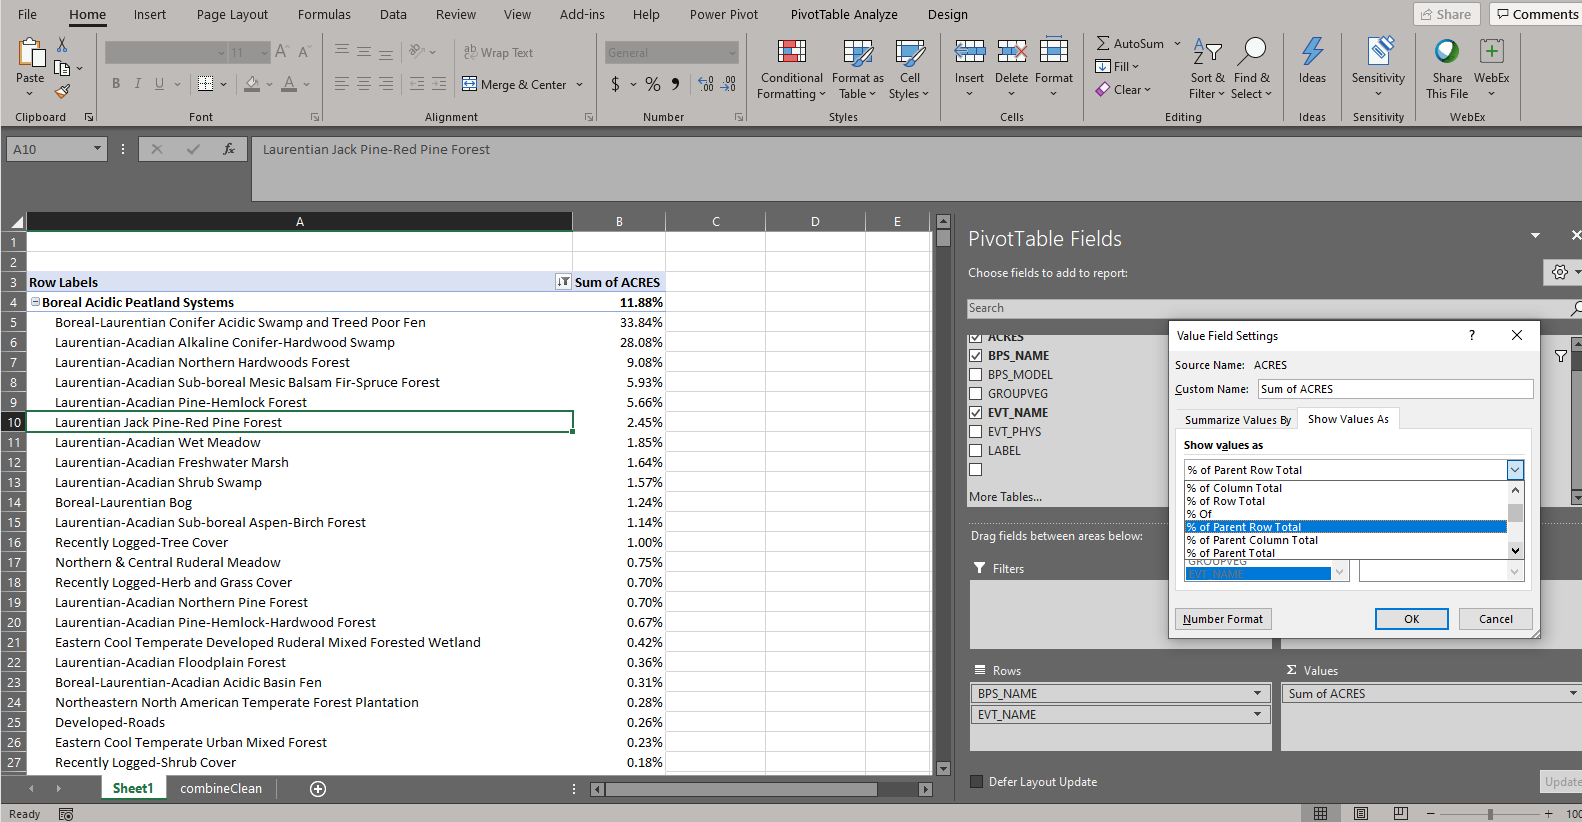
\includegraphics[width=1\linewidth]{pivotPercentParent}

You'll see that \textasciitilde34\% of what was classified as ``Boreal Acidic Peatland Systems'' in the BpS dataset for our landscape is now classified as ``Boreal-Laurentian Conifer Acidic Swamp and Treed Poor Fen'' in the Existing Vegetation Type dataset. Scroll through the table below to explore the resulting data. The table has been exported from the Pivot Table and cleaned up a bit for viewing.

\textbf{Note: I filtered for the Top 10 EVTs per BpS.}

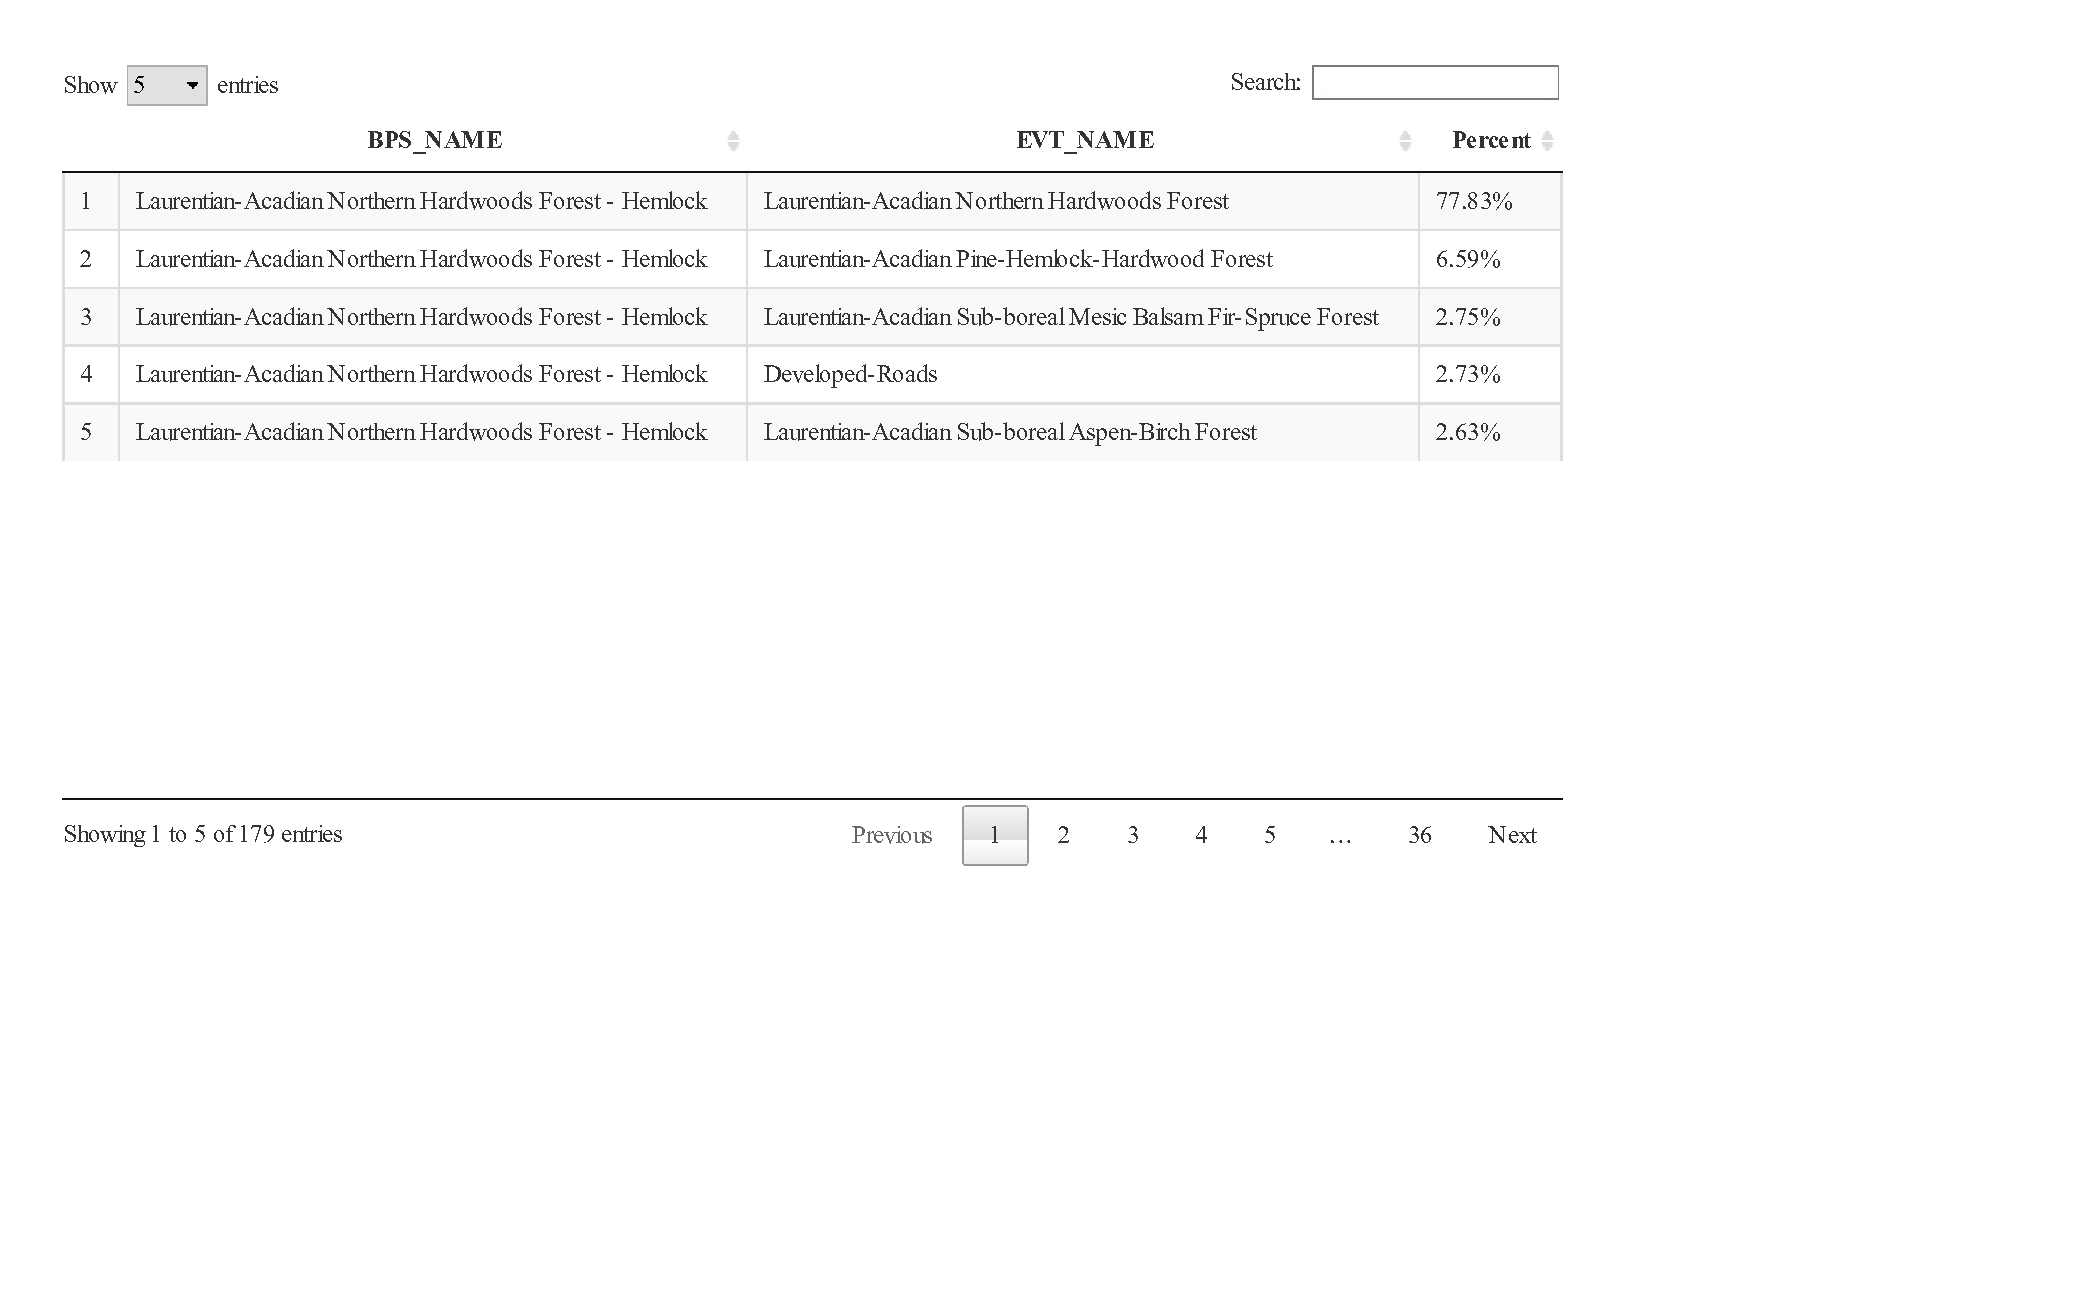
\includegraphics{FSCBook_files/figure-latex/bpsEvtDT-1.pdf}

Looking at the Laurentian-Acadian Northern Hardwoods Forest - Hemlock for our landscape we note a few things:

\begin{itemize}
\tightlist
\item
  Most of what was mapped as this type historically in the BpS dataset is still mapped as that type
\item
  Cumulatively about 6\% of this type is now roads and recently logged types.
\item
  The other EVTs mapped are not terribly ``off-site'' (e.g., something like ``Plantation'').
\end{itemize}

\hypertarget{the-fine-print}{%
\section{The fine print}\label{the-fine-print}}

While this assessment is illustrative, it is important to note that the methods used to create the BpS and EVT datasets are substantially different, and LANDFIRE datasets are not made for assessing small areas. Please review.

\hypertarget{histDist}{%
\chapter{Historical Disturbance Regimes}\label{histDist}}

Getting at historical disturbance regimes.

Need reviewed BpS model output spreadsheet.

\hypertarget{final-words}{%
\chapter{Final Words}\label{final-words}}

We have finished a nice book.

\end{document}
